\documentclass[../main.tex]{subfiles}

\begin{document}

\section{Modeling with exponential functions}

During the last sessions we where focused on the porperties of the functions, that is, the range of the function, translations of the function in the $x$ and $y$ axis, the inverse function, asymptotes and critical points.
Now we are going to use all of that knowledge to describe idealized natural phenomena, such as, population growth, radioacive decay, heat diffusion and others.
As the title of the topic suggest, we are going to use exponential functions to model idealized natural phenomena.
Bellow is a recap of the properties of the exponential function and usefull characteritics which will be usefull later on.
\begin{definition}{Exponential function}{exp-fun-def}
    An exponential function is represented as follows,
    \begin{gather*}
        f(x) = a^x,
    \end{gather*}
    where $a>0$, $a\neq1$ and is refere as the ``base''.
    Has domain in all the real numbers ($x\in\mathbb{R}$ or $x\in\qty(-\infty,\infty)$) and range in the positive real numbers ($f(x)\in\qty(0,\infty)$).
    Also has a horizontal asymptote at $y = 0$.

    %\begin{figure}[ht!]
    \centering
        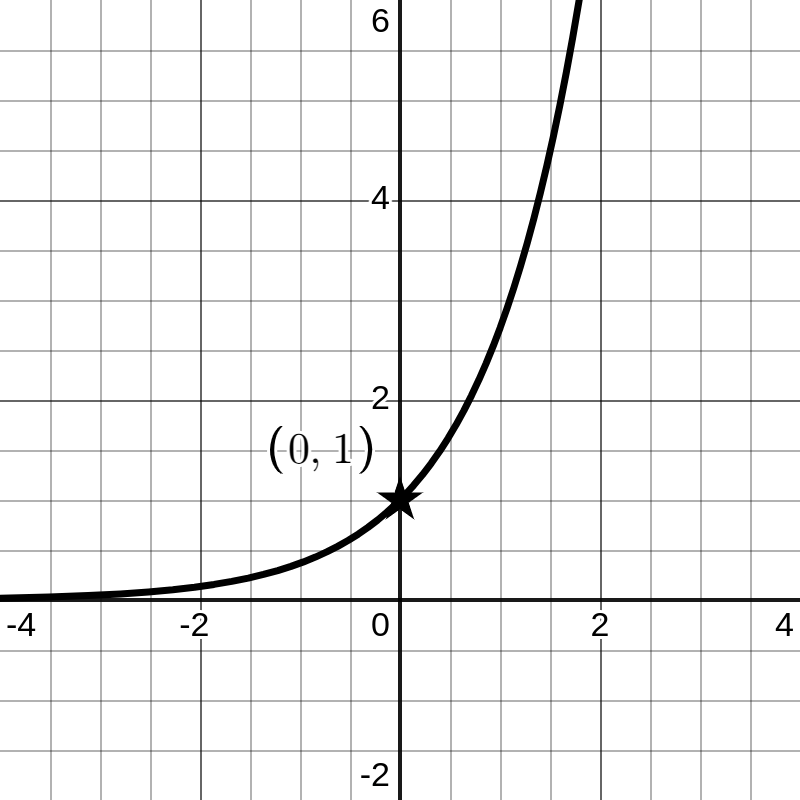
\includegraphics[width=0.4\textwidth]{imgs/exp-graph.png}
    
    %\end{figure}
\end{definition}

We can modify the function by adding the following parameters, $n_o,~r,~x_o$ and $f_o$,
\begin{gather*}
    f(x) = n_o a^{r\qty(x-x_o)} + f_o.
\end{gather*}
The parameter $n_o$ modifies the intersection with the $y$ axis.
The parameter $r$ controls how ``\textit{quickly}'' the function grows or decreases.
The parameter $x_o$ moves the function to the left or right and the parameter $f_o$ shifts the horizontal asymptote up or down.
As a recommendation, try to plot in desmos an exponential function with those paramenters and play with them to see the transformations.

\subsection{Common type of exponential growth}

From the definition of the exponential function, we can see that function is mainly defined by the base ``$a$''.
Using that fact, the following example is going to take into account natural phenomena that can be model with exponential functions with base $e$.

\begin{comment}
\begin{definition}{Exponential growth (Doubling time)}{exp-label1}
    If the initial size of a population is $n_o$ and the doubling time is $a$, then the size of the population at time $t$ is
    \begin{gather*}
        n(t) = n_o 2^{t/a}
    \end{gather*}
    where $a$ and $t$ are measured in the same time unit (minutes, hours, days, years, and so on).
\end{definition}
\end{comment}

\begin{definition}{Exponential growth (Relative growth rate)}{exp-label2}
    A population that experiences exponential growth increases acording to the model
    \begin{gather*}
        n(t) = n_o e^{rt}
    \end{gather*}
    where, $n(t)$ is the population at time $t$, $n_o$ is the initial size of the population, $r$ is the relative rate of growth (typically expressed as a proportion of the population) and $t$ represents time.
\end{definition}

\begin{example}{Predicting the Size of a Population}{}
    Lets consider an initial bacterium count in a culture is \num{500}.
    Half an hour later a biologist makes a sample count of bacteria in the culture and finds that the count in the culture is approximately \num{610}.
    \begin{enumerate}[label=(\alph*)]
        \item Find a function that models the number of bacteria after $t$ hours.
        \item What is the estimated count after $10$ hours?
        \item After how many hours will the bacteria count reach \num{80000}?
    \end{enumerate}

    \paragraph{(a)} We know, that we can model the size of a populetion with the following function \[n(t)=n_oe^{rt}.\]
    Therefore, we need to find the parameters $n_o$ and $r$.
    Recalling the properties of the exponential functions, when the function is evaluated at $t=0$, we get the constant $n_o$,
    \begin{align*}
        n(0) &= n_o e^{r\cdot0} \\
        500 &= n_o \cdot 1 \\
        500  &= n_o.
    \end{align*}

    Now, we can focus into the parameter $r$.
    To do that, we are going to substitute the values given by the second condition, $n(0.5) = \num{610}$,
    \begin{align*}
        n(0.5) &= 500 e^{r\cdot 0.5} \\
        \cancelto{1.22}{\frac{610}{500}} &= e^{r\cdot 0.5} \\
        \ln\qty[1.22] &= \ln\qty[e^{r\cdot 0.5}] \\
        \ln\qty[1.22] &= \qty(r\cdot 0.5)\cancelto{1}{\ln\qty[e]} \\
        \frac{\ln\qty[1.22]}{0.5} &= r \\
        0.397701 &= r.
    \end{align*}
    Therefore, the function that models the number of bacteria after $t$ hours is \[n(t)=500e^{0.397701\cdot t}.\]

    \paragraph{(b)} Now that we know the function, we evaluate the function at $t=10$,
    \begin{align*}
        n(10) &=500e^{0.397701\cdot 10} \\
              &\simeq \num{26678.628640}
    \end{align*}

    \paragraph{(c)} Finally, we need to find the time at which the population will reach a bacterium count of \num{80000} ($n(t)=\num{80000}$).
    To do that, we simply substitute the value of the function and solve for  $t$,
    \begin{align*}
        n(t) &= 500e^{0.397701\cdot t} \\
        \num{80000} &= 500e^{0.397701\cdot t} \\
        \cancelto{160}{\frac{\num{80000}}{500}} &= e^{0.397701\cdot t} \\
        \ln\qty[160] &= \ln\qty[e^{0.397701\cdot t}] \\
        \ln\qty[160] &= \qty(0.397701\cdot t)\cancelto{1}{\ln\qty[e]} \\
        \ln\qty[160] &= 0.397701\cdot t \\
        \frac{\ln\qty[160]}{0.397701} &= t \\
        \num{12.761279} &\simeq t.
    \end{align*}
    Which tells us that the bacterium culture will reach a bacterium count of \num{80000} after \num{12.761} hours.


\end{example}

\subsection{Excersices}

The element Polonium-210 ($^{210}\mathrm{Po}$) has a half-life of \num{140} days, that is, $m(140) = m_o/2$.
Suppose a sample of this element has a mass of \SI{300}{\milli\gram}.
\begin{enumerate}[label=(\alph*)]
    \item Find a function that models the mass remaining after $t$ hours.
    \item Find te mass remaining after \num{300} days. 
    \item How long will it take the sample to decay to a mass of \SI{75}{\milli\gram}?
\end{enumerate}

\end{document}
